% Options for packages loaded elsewhere
\PassOptionsToPackage{unicode}{hyperref}
\PassOptionsToPackage{hyphens}{url}
%
\documentclass[
]{book}
\usepackage{lmodern}
\usepackage{amssymb,amsmath}
\usepackage{ifxetex,ifluatex}
\ifnum 0\ifxetex 1\fi\ifluatex 1\fi=0 % if pdftex
  \usepackage[T1]{fontenc}
  \usepackage[utf8]{inputenc}
  \usepackage{textcomp} % provide euro and other symbols
\else % if luatex or xetex
  \usepackage{unicode-math}
  \defaultfontfeatures{Scale=MatchLowercase}
  \defaultfontfeatures[\rmfamily]{Ligatures=TeX,Scale=1}
\fi
% Use upquote if available, for straight quotes in verbatim environments
\IfFileExists{upquote.sty}{\usepackage{upquote}}{}
\IfFileExists{microtype.sty}{% use microtype if available
  \usepackage[]{microtype}
  \UseMicrotypeSet[protrusion]{basicmath} % disable protrusion for tt fonts
}{}
\makeatletter
\@ifundefined{KOMAClassName}{% if non-KOMA class
  \IfFileExists{parskip.sty}{%
    \usepackage{parskip}
  }{% else
    \setlength{\parindent}{0pt}
    \setlength{\parskip}{6pt plus 2pt minus 1pt}}
}{% if KOMA class
  \KOMAoptions{parskip=half}}
\makeatother
\usepackage{xcolor}
\IfFileExists{xurl.sty}{\usepackage{xurl}}{} % add URL line breaks if available
\IfFileExists{bookmark.sty}{\usepackage{bookmark}}{\usepackage{hyperref}}
\hypersetup{
  pdftitle={BABLab Manual},
  hidelinks,
  pdfcreator={LaTeX via pandoc}}
\urlstyle{same} % disable monospaced font for URLs
\usepackage{longtable,booktabs}
% Correct order of tables after \paragraph or \subparagraph
\usepackage{etoolbox}
\makeatletter
\patchcmd\longtable{\par}{\if@noskipsec\mbox{}\fi\par}{}{}
\makeatother
% Allow footnotes in longtable head/foot
\IfFileExists{footnotehyper.sty}{\usepackage{footnotehyper}}{\usepackage{footnote}}
\makesavenoteenv{longtable}
\usepackage{graphicx,grffile}
\makeatletter
\def\maxwidth{\ifdim\Gin@nat@width>\linewidth\linewidth\else\Gin@nat@width\fi}
\def\maxheight{\ifdim\Gin@nat@height>\textheight\textheight\else\Gin@nat@height\fi}
\makeatother
% Scale images if necessary, so that they will not overflow the page
% margins by default, and it is still possible to overwrite the defaults
% using explicit options in \includegraphics[width, height, ...]{}
\setkeys{Gin}{width=\maxwidth,height=\maxheight,keepaspectratio}
% Set default figure placement to htbp
\makeatletter
\def\fps@figure{htbp}
\makeatother
\setlength{\emergencystretch}{3em} % prevent overfull lines
\providecommand{\tightlist}{%
  \setlength{\itemsep}{0pt}\setlength{\parskip}{0pt}}
\setcounter{secnumdepth}{5}
\usepackage{booktabs}
\usepackage{amsthm}
\makeatletter
\def\thm@space@setup{%
  \thm@preskip=8pt plus 2pt minus 4pt
  \thm@postskip=\thm@preskip
}
\makeatother
\usepackage[]{natbib}
\bibliographystyle{apalike}

\title{BABLab Manual}
\author{}
\date{\vspace{-2.5em}}

\begin{document}
\maketitle

{
\setcounter{tocdepth}{1}
\tableofcontents
}
\hypertarget{callaghan-brain-and-body-lab-manual}{%
\chapter{Callaghan Brain and Body Lab Manual}\label{callaghan-brain-and-body-lab-manual}}

\begin{figure}
\centering
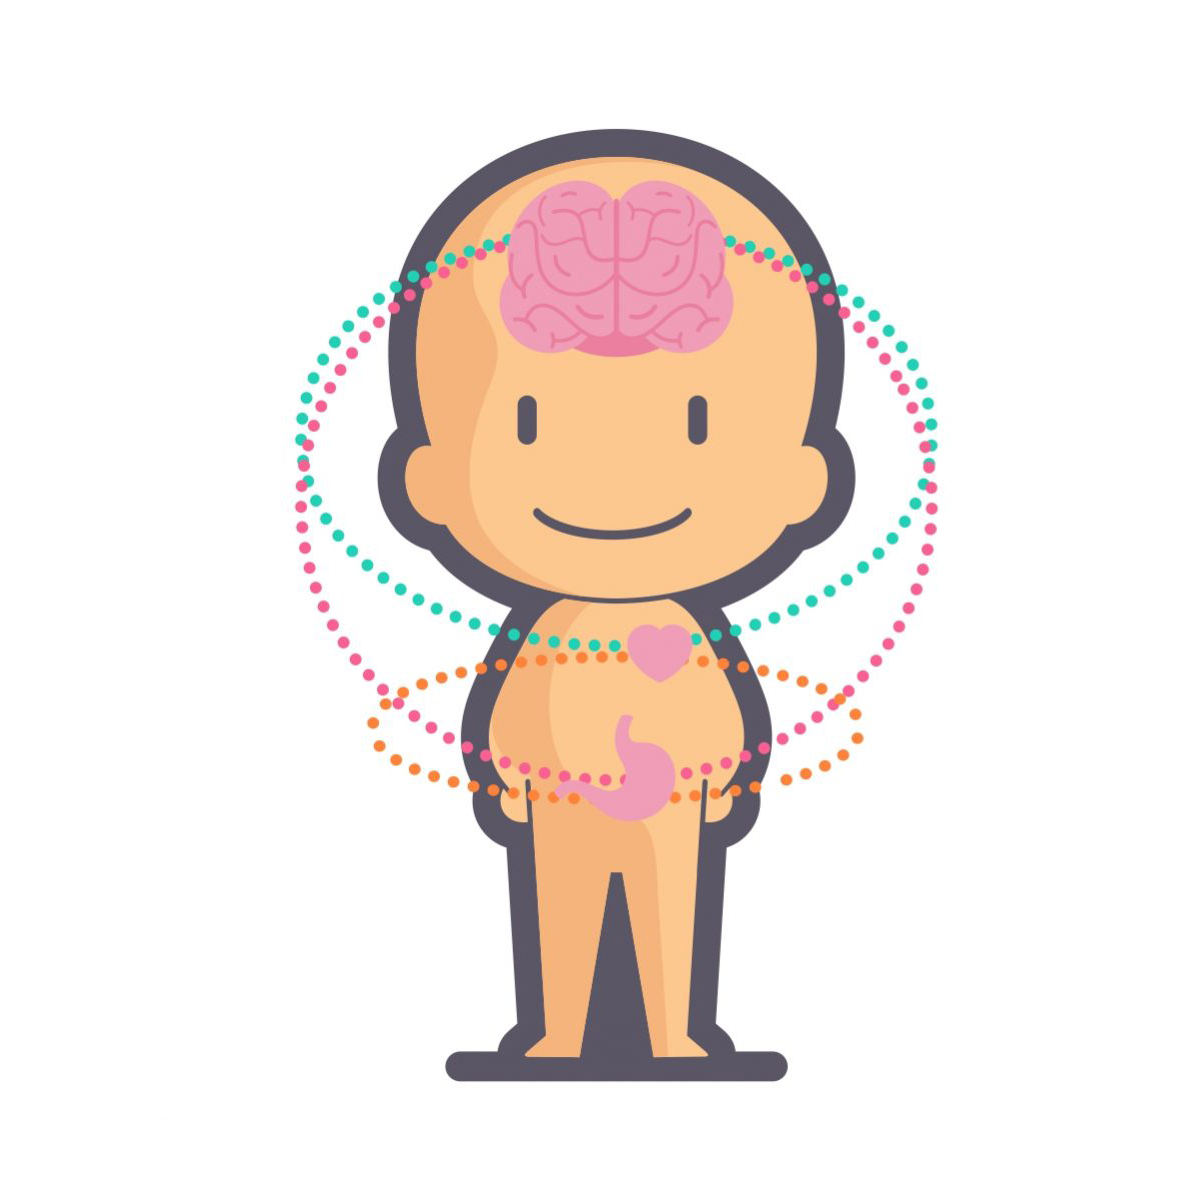
\includegraphics[width=0.5\textwidth,height=0.5\textheight]{images/index/Icon.jpg}
\caption{}
\end{figure}

\hypertarget{welcome}{%
\section{Welcome}\label{welcome}}

\begin{center}\rule{0.5\linewidth}{0.5pt}\end{center}

Welcome to the Brain and Body Lab at UCLA!

We are so glad that you are joining us, in whatever capacity it is (undergraduate, research assistant, graduate student, postdoc, visiting scholar, or collaborator). Academia can be a confusing place, and no two labs are the same. We have written this manual to make your transition into the BABLab as smooth as possible, to share the goals of the lab, its inner workings, as well as its unique culture, to which you will contribute. We hope that during your time here, you will learn a lot about the brain and its interactions with the rest of the body, about developmental psychology, and about science in general. It is our collective goal to have everyone leave the lab with more than they started with, should that be new skills, a fresh perspective or understanding on a given topic, and a network of colleagues and friends. We hope that you make it your goal to place your own positive stamp on the lab, and to contribute to it in a meaningful way. Just like us, a lab grows and develops over time, and each individual shapes its path. We look forward to seeing what your time in the lab will bring.

This lab manual was inspired by several others, and borrows heavily from them (e.g., \href{https://github.com/alylab/labmanual/blob/master/aly-lab-manual.pdf}{this one} by the Aly Lab and \href{https://github.com/memobc/memolab-manual}{this one} from the Ritchey Lab were the primary sources and the main template I used. A little of \href{https://github.com/jpeelle/peellelab_manual/blob/master/peellelab_manual.pdf}{this one} too).

A lot of time was put into the creation of this document. Thinking about what we want our lab to be, what are we going to be known for, and how can we make this lab work for everyone. We really respect the principles and ideas we are aspiring to here, and for that reason, we ask that all new lab members read the manual in full.

\emph{This lab manual is licensed under a \href{https://creativecommons.org/licenses/by-nc/4.0/}{Creative Commons Attribution - NonCommercial 4.0 International License}. If you want to make your own manual for a lab, or any other purpose, please feel free to take any ideas and inspiration for this one (and cite us), as well as from the others we have used when making this (and cite them).}

\begin{center}\rule{0.5\linewidth}{0.5pt}\end{center}

\hypertarget{mission-statement}{%
\section{Mission Statement}\label{mission-statement}}

In the BABLab we aim to do good science that makes a difference. That is our mission. To do it, we need people to be passionate about what we are doing and come to work in a good frame of mind to get it done. We aim to be nurturing, challenging, and stimulating to students. We aim to be respectful, engaging, and meaningful for families and participants.

\begin{center}\rule{0.5\linewidth}{0.5pt}\end{center}

\hypertarget{diversity-commitment}{%
\section{Diversity Commitment}\label{diversity-commitment}}

We in the BABLab value the diversity of our lab members and research participants. We take seriously our role as allies for Indigenous, Black, and Communities of Color, and are committed to learn, understand, and dismantle systems of oppression, particularly in academia. You are welcome in this lab whatever the color of your skin, your sexual orientation, and your gender identity. Read on for some of the concrete steps we are taking in the lab to address racism and encourage diversity in the 2020-2021 academic year.

\begin{enumerate}
\def\labelenumi{\arabic{enumi}.}
\item
  We will continue to support historically underrepresented students through the PROPS program at UCLA.
  If you are a junior or senior in Psychology at UCLA, consider applying to the PROPS program for a research intensive experience. \url{https://www.psych.ucla.edu/undergraduate/special-programs-and-events/psychology-research-opportunities-programs/props-application}
\item
  Diversity focused lab meetings.
  Across the Summer of 2020 we trailed a new format of lab meeting focused on diversity in academia. These are be meetings where we amplify black and brown voices and discuss issues of race and racism in science and academia. Going forward in 2020 and into 2021, we are making a commitment to be mindful of the diversity of samples in papers that we review and to think about how sample diversity and the questions that were asked influence findings.
\item
  Engaging in more Community Based Participatory Research.
  It is our mission in the BABLab to make a difference in people's lives through the work we do. It is hard for our work to make a difference when the community is not actively involved in the research process from start through finish, not as `subjects' or `participants', but as partners. We have been working on creating lasting and meaningful community partnerships since our inception in 2019. As a concrete step forward in this same direction, we commit to including a timeline and dedicated funds to establish a Community Advisory Board for all future community facing grants.
\item
  Reviving and refreshing each new academic year.
  The world we live in changes rapidly, and practices become quickly outdated and superseded. We in the BABLab are making a commitment to review our diversity statement and practices at the beginning of every academic year, checking in with the students and staff to see what is working and not working for them, and making adjustments where necessary.
\end{enumerate}

\hypertarget{expectations-and-responsibilities}{%
\chapter{Expectations and Responsibilities}\label{expectations-and-responsibilities}}

\begin{center}\rule{0.5\linewidth}{0.5pt}\end{center}

\hypertarget{everyone}{%
\section{Everyone}\label{everyone}}

Big Picture

Sometimes science can be hard, and the rewards (amazing research findings, papers, etc.) can be few and far between. However, science is always fun when we make the lab a great place to me. In the BABLab, we want everyone to have a positive experience that is free from hostility, so that people can do their best, most productive science. Great labs don't just happen, they are built. Here is what we can all do to help:

\begin{itemize}
\tightlist
\item
  Do work that you are proud of.
\item
  Work carefully, and strategically. Do not rush.
\item
  Respect our participants. Whether they are families, undergrads, our adults from the community, they are giving up their time to be involved in research. Always act professionally with participants over the phone and in person, do not leave them waiting. Keep in mind that participants may have different political and religious beliefs, sexual orientations, family compositions, and have had very different life experiences, to you and/or your friends. Please do conduct yourself in a way that respects their unique situation and personhood.
\item
  Respect our child participants. In addition to the above point, remember that children are to be respected as much as adults. Please be aware that even well-meaning adults can sound patronizing sometimes when speaking with children. At the risk of sounding patronizing myself, comments like ``cool dress'' or ``neat sneakers'' are fine, but comments like ``you are so cute'' could come off as patronizing.
\item
  Respect the data and the people who collected it. Data collection, especially in developmental populations, is hard. People put their blood, sweat, and tears into it. They came in on weekends, after hours, on holidays, in rain, hail, and shine (mostly shine -- because, Cali) to get it. You might be analyzing data that you did not have to collect. That is a pretty great situation, so make sure you treat that data in the same way you would your own.
\item
  Respect your lab mates: their culture, religion, beliefs, sexual orientation, and personality quirks. Science is for everyone.
\item
  Respect yourself: your need for time off, your happiness, your other commitments. You are responsible for constructing your boundaries.
\item
  Be supportive of your lab mates: We are a team. Science is about collaboration, not competition.
\item
  Be forgiving of yourself and one another. Being in an academic environment can be challenging. We all make mistakes, and not everyone is on their A-game every day. Whatever happens, try to be understanding, forgive, and move on.
\item
  Tension or hostility in the lab affects everyone and behaving in a bullying, intimidating, rude or disrespectful way will not be tolerated. I expect everyone to be mature and professional while in the lab, this is a workplace and should be treated in that way. If there are any problems which cannot be dealt with in the lab, please tell Bridget.
\item
  Be honest with yourself and others. This means that if you notice a mistake, however embarrassing, admit it, correct it, and move on.
\item
  Check everything several times. Then get someone else to check it. Then check it again. It's ok to makes mistakes, but mistakes shouldn't be because of carelessness or rushed work.
\item
  Under no circumstances is it ok to plagiarize, tamper with data, make up data, or omit data. If you are feeling pressured to succeed and think that is interfering with your judgement, you should reach out to Bridget and we can talk about it. However, pressure is something we all face and is not an excuse to engage in academic misconduct.
\item
  If you are struggling with health and/or unhappiness, or if you see someone else that is struggling, please come and see me (Bridget). Everyone goes through rough patches, and we want to help each other out.
\item
  Have a life outside of the lab, take care of your mental and physical health, and don't ever feel bad for taking time off work, and don't make others feel bad for doing that either.
\end{itemize}

Small Picture

There are a few day-to-day things to keep in mind to keep the lab running smoothly.

\textbf{Special considerations for virtual format during the covid-19 pandemic}

\begin{itemize}
\tightlist
\item
  The lab is now collecting data online. Please be aware of what you are wearing in the online environment and make sure that it is respectable and that your surroundings are respectable.For instance, if you are with participants, you should be in a non distracting background. We understand that you can't choose where you're working from at this time, so please do this within the constraints of your individual situation.
\item
  When we do have a common lab space in which we meet, it is even more important to check slack and email on a regular basis and be available to respond to messages, set up virtual meetings, etc.
\end{itemize}

\textbf{general}:

\begin{itemize}
\tightlist
\item
  If you're sick, please take time off, stay home (if we are in person), and take care of yourself. Just slack the lab manager or me (Bridget) to tell us. Because you need it, and also because others don't need to get sick.
\item
  If you know you might be sick, e.g., you have a minor surgery and don't know how well you will recover, play it safe and reschedule your appointments ahead of time.
\item
  Working in developmental populations means that work times need to be flexible. If you are collecting data or recruiting participants, you may be expected to work on weekends and holidays. We will make a schedule to share that burden as evenly as possible. When you collect data or recruit participants outside of work hours, I expect that you will take some time off during work hours to compensate.
\item
  Outside of data collection and recruitment, you are not expected to work or come into the lab (if we are in person) on weekends or holidays, and you are not expected to stay late at night.
\item
  You are expected to get your work done to a high standard and you can do that in whatever time of day best suits you and your work style. That being said, being in lab some of the time is important for the lab, and for morale, so you shouldn't work remotely all of the time (unless we are in a pandemic). (Note: the lab manager is expected to keep more regular hours than other lab members: 8am-5pm, 9am-6pm, 10am-7pm are all reasonable work hours for a lab manager).
\item
  All grad students, post-docs, and paid employees (e.g., lab managers, research associates, and technicians) are expected to attend lab meetings when their schedules allow. We will set a time for the lab meeting each term that best fits everyone's schedule.
\item
  Volunteers in the lab and other students are expected to attend lab meeting when it suits their schedule and when it is of interest to them.
\item
  Make sure the door to the lab is locked if no one is inside. Turn off the lights if you're the last one leaving for the day. And water the plants if they are looking sad.
\item
  Keep the lab tidy. Eating in lab is fine, but clean up food waste, crumbs, spills. Put lab equipment back where you found it. Keep common areas uncluttered.
\item
  Lab is a shared space. Unless you have been assigned a permanent desk, do not permanently claim a space. Use space when it is available and remove your belongings when you leave so that others can use the space.
\item
  Dress code is casual, neat, and approachable. When interacting with participants or presenting your work, don't wear pajamas, dirty clothes, clothes with holes in them, or clothes that are see-through. Jeans are totally fine and even sweatpants/active wear is fine when you are in the lab and collecting data. Remember that when you are collecting data, it will mostly be with kids, so we want to be approachable and comfortable (you might end up on the floor), keep that in mind when considering what to wear. If you want to dress up, that is fine too - as long as you are comfortable and approachable.
\item
  When you are running participants show up 15-20 minutes early to set everything up.
\item
  Be on time for your meetings: respect that others have busy schedules and everyone's time is valuable.
\item
  Last of all, we all have unique ways of working. I (Bridget) have written a `user manual' so that you can be familiar with mine. Please read it, so that you get to know me a little better from the outset and we can avoid misunderstandings.
\end{itemize}

\begin{center}\rule{0.5\linewidth}{0.5pt}\end{center}

\hypertarget{principal-investigator}{%
\section{Principal Investigator}\label{principal-investigator}}

All of the above, and I will\ldots{}

\begin{itemize}
\tightlist
\item
  Support your scientific development and be responsive to your emotional needs
\item
  Give you feedback on a timely basis, including feedback on project ideas, conference posters, talks, manuscripts, figures, grants
\item
  Be available in person and via slack on a regular basis, including regular meetings to discuss your research
\item
  Support your career development in whatever way I can (e.g., by introducing you to other researchers in the field, promoting your work at talks, writing recommendation letters for you, and letting you attend conferences as often as finances permit)
\item
  Help you prepare for the next step of your career, whether it's a post-doc, a faculty job, or a job outside of academia
\end{itemize}

\begin{center}\rule{0.5\linewidth}{0.5pt}\end{center}

\hypertarget{post-docs}{%
\section{Post-Docs}\label{post-docs}}

All of the above, and you will also be expected to\ldots{}

\begin{itemize}
\tightlist
\item
  Develop your own independent line of research
\item
  Collect data for ongoing projects in the lab, including any group projects. Although the data collection responsibilities of postdocs are lower than others in the lab, taking part in data collection for group projects is everyone's responsibility
\item
  Write and submit scientific papers (including review papers) in a timely manner
\item
  Help train and mentor students in the lab (both undergraduate and graduate)
\item
  Seek out opportunities to present your work (e.g., at departmental events, in other labs, and at conferences)
\item
  Engage in networking opportunities (e.g., chair a symposium, attend other lab meetings, volunteer as a student representative at conferences)
\item
  Apply for grants (e.g., NRSA, K99, NARSAD). Writing grants is an excellent exercise to find direction in your research, and identify gaps in your training that you can address. It will also give you greater autonomy in the lab, will help your CV, and will help the lab (by freeing up funds, as well as providing a model for the other students to follow). Please see Bridget early about finding different grant mechanisms to apply for, and for example grants
\item
  Apply for jobs (academic or otherwise) when you're ready, or after you have discussed your progress with Bridget. Postdoctoral training can lead to many different jobs, some in academia, industry and elsewhere. Any of those paths are fine with me (Bridget). Please keep me abreast of your thinking around potential jobs and I will support your career goals in whatever way I can
\end{itemize}

\begin{center}\rule{0.5\linewidth}{0.5pt}\end{center}

\hypertarget{graduate-students}{%
\section{Graduate Students}\label{graduate-students}}

All of the above, and you will also be expected to\ldots{}

\begin{itemize}
\tightlist
\item
  Develop your dissertation research. This includes knowing the literature like the back of your hand. Take ownership of your project and treat it like your baby
\item
  Collect data for the ongoing projects in the lab, which includes any major group projects
\item
  Help mentor undergraduate students in the lab
\item
  Seek out opportunities to present your work (e.g., at departmental events, in other labs, and at conferences)
\item
  Engage in networking opportunities (e.g., attend other lab meetings, volunteer as a student representative at conferences)
\item
  Apply for grants (e.g., NRSA, NSF). Writing grants is an excellent exercise to find direction in your research, and identify gaps in your training that you can address. It will also free up your time from Teaching Assistant (TA) commitments
\item
  Think critically about what you want for your career (academia -- research or teaching, industry, science writing, something else). It is never too early to start discussing this with me (Bridget) so that we can make sure you are getting the types of training you need
\item
  Make sure you meet all departmental and internal lab deadlines (e.g., for your exams and thesis) -- and make sure Bridget is aware of them!
\item
  Prioritize time for research. Coursework and TA'ing are important, but it is research that matters for the PhD.
\end{itemize}

\begin{center}\rule{0.5\linewidth}{0.5pt}\end{center}

\hypertarget{lab-managers}{%
\section{Lab Managers}\label{lab-managers}}

All of the above, and you will also be expected to\ldots{}

\begin{itemize}
\tightlist
\item
  Collect data for the ongoing group projects in the lab
\item
  Manage the lab's data backup and ensure backups are done on a consistent basis
\item
  Work on your own research (developed with Bridget's help) that will either be a review paper, analysis of an existing data set, a study within the group project, or another project that sits outside the group project
\item
  Create research and lab protocols
\item
  Train new lab members on the research and lab protocols
\item
  Monitor adherence to research and lab protocols
\item
  Hire, train, mentor, and assess progress of undergraduate research assistants. This includes setting them up with access to the lab, making sure they have properly onboarded, and making sure they are included in the IRB protocols they are working on
\item
  Schedule and manage the work of undergraduate research assistants
\item
  Maintain IRB protocols for the lab (writing them, renewing them), archive old consent forms, keep any required paperwork up to date and organized
\item
  Maintain the lab website and lab wiki, update the lab manual, add lab events to the lab calendars, manage the lab server, check and respond to the lab e-mail address (\href{mailto:bablab.ucla@gmail.com}{\nolinkurl{bablab.ucla@gmail.com}}).
\item
  Give new lab members access to the lab wiki, lab GitHub, lab calendars, and add their experiments to the lab server.
\item
  Assist with the recruitment and scheduling of participants for the group project, and for the smaller projects in the lab
\item
  Help to manage grant budgets and startup funds
\item
  Monitor lab supplies (e.g., toner and paper for the printer, books for students) and order more supplies when needed
\end{itemize}

\begin{center}\rule{0.5\linewidth}{0.5pt}\end{center}

\hypertarget{senior-research-assistants}{%
\section{Senior Research Assistants}\label{senior-research-assistants}}

All of the above, and you will also be expected to\ldots{}

\begin{itemize}
\tightlist
\item
  Help collect data for the lab's projects, including running participant sessions
\item
  Recruit new participants for the lab's research
\item
  Handle communication with enrolled participants, including scheduling, reminders, session confirmations, etc.
\item
  Attend lab meetings and/or RA meetings when it fits your schedule and if you have interest
\item
  Attend a weekly meeting with the lab manager and all SRAs
\item
  Update the Availability calendar and communicate with the lab manager regarding your schedule for lab work and availability for participant sessions
\end{itemize}

\begin{center}\rule{0.5\linewidth}{0.5pt}\end{center}

\hypertarget{enrolled-research-interns}{%
\section{Enrolled Research Interns}\label{enrolled-research-interns}}

All of the above, and you will also be expected to\ldots{}

\begin{itemize}
\tightlist
\item
  Develop your own research project in the lab
\item
  Complete your work in a timely manner and make sure you back up your work, and file it appropriately within the lab server (generally, until you have final versions, this will be in your user folder on Box).
\item
  Make sure that your work is accessible to anyone. That is, comment your code, name files appropriately (see wiki for lab file naming conventiosn), document all aspects of your project, and create a wiki with all important information.\\
\item
  Meet regularly with Bridget or whoever is your assigned mentor to discuss your project
\item
  Attend lab meetings and RA meetings when it fits your schedule and if you have interest
\item
  Once you have finalized a piece of work (e.g., script, wiki), send it to the lab manager for approval. Once it has been approved, the lab manager will copy it to main study folder on Box.
\item
  Note that if you would like to also work as a research assistant in the lab, you must meet with Bridget first. Also please understand that those duties will require a 10 hour per week commitment (separate from anything you are doing for your research project).
\end{itemize}

\begin{center}\rule{0.5\linewidth}{0.5pt}\end{center}

\hypertarget{research-assistants}{%
\section{Research Assistants}\label{research-assistants}}

All of the above, and you will also be expected to\ldots{}

\begin{itemize}
\tightlist
\item
  Assist other lab members with data collection and analysis
\item
  Work on any projects that your lab mentor has given you
\item
  Complete your work in a timely manner and make sure you back up your work, and file it appropriately within the lab server.
\item
  Make sure that your work is accessible to anyone. That is, leave notes explaining what was done, make sure that spreadsheets and any color coding you used in them are properly annotated
\item
  Develop your weekly schedule by talking to your graduate student mentor or your post-doc mentor. You should be coming in every week, and scheduling enough time to get your work done
\item
  Attend lab meetings when it fits your schedule and if you have interest
\item
  Attend RA meetings
\item
  Keep a log of the work you did in the lab, the dates you were in the lab, and the hours you worked. Send this to your lab mentor when you finish up in the lab. They will use this to write you a letter of reference
\end{itemize}

\hypertarget{code-of-conduct}{%
\chapter{Code of Conduct}\label{code-of-conduct}}

\begin{center}\rule{0.5\linewidth}{0.5pt}\end{center}

\hypertarget{essential-policies}{%
\section{Essential Policies}\label{essential-policies}}

Student Conduct Code

UCLA has a Student Conduct Code which can be found \href{https://www.deanofstudents.ucla.edu/Individual-Student-Code}{here}. Please take the time to familiarize yourself with it before you start in the lab.

\begin{center}\rule{0.5\linewidth}{0.5pt}\end{center}

\hypertarget{scientific-integrity}{%
\section{Scientific Integrity}\label{scientific-integrity}}

Reproducible Research

The BABLab at UCLA is committed to performing reproducible research. Reproducible research means that, if you gave someone your raw data and analysis code they should be able to reproduce your results exactly. If they can't it suggests that something is wrong (e.g., there is a mistake in the pipeline) or that you did not properly document the data collection, cleaning, or analysis process. Neither of these options is good. Therefore, we take steps towards ensuring that all aspects of the data collection, cleaning, and analysis are extremely well documented.

For results to be reproducible, you need to be organized and document everything! Take detailed notes on your study design, make sure you save all of the citations for questionnaires you use, if you make up a questionnaire yourself, document that it was made for the study, so that you or someone else doesn't spend hours looking for the citation later on down the track, thinking it was a validated measure. Keep notes on the different recruitment methods, inclusion/exclusion criteria, participant schedule for study days, all the research protocols, as well as any changes to the protocols that occur during the study. If something goes wrong, or something unusual happens, document that too. Document the parameters for the MRI scanner, document the versions of the software used to collect the data. Before you start collecting data, you should aim to have a private OSF project, or study that forks to the main project, that is as detailed as this example from the Child Mind Institute.

Once you have collected data, you need to take detailed notes on data cleaning and analysis. Even if you have preregistered your study design (which you very likely will do), you still need to document this stage, as you may move away from your preregistered cleaning and analysis choices for a variety of reasons. You need to know what those reasons are. You need to write down how you did things every step of the way (and the order that you did things), from any pre-processing of the data, to running models, to statistical tests. Additionally, your code should also be commented, and commented clearly. We all know what it's like to sit down, quickly write a bunch of code to run an analysis without taking time to comment it, and then having no idea what we did a few months down the road. Comment your code so that every step is understandable by an outsider. Finally, it is highly encouraged that you use some form of version control (e.g., Git in combination with GitHub) to keep track of what code changes you made and when you made them, as well as sharing code with others.

In sum, you should write copious notes on your study design and all of the measures before you start the study and place every bit of information on OSF (you will likely also be preregistering your study on OSF). Then you should write beautifully annotated code to clean and analyze your data (e.g., use R-Markdown) and then place that on GitHub. There is nothing more satisfying in science (or life) than a well-organized study. Your future self will thank your current self, and everyone in the lab will thank you too.

Authorship

Like other labs, we will follow the APA guidelines with respect to authorship:

\begin{quote}
``Authorship credit should reflect the individual's contribution to the study. An author is considered anyone involved with initial research design, data collection and analysis, manuscript drafting, and final approval. However, the following do not necessarily qualify for authorship: providing funding or resources, mentorship, or contributing research but not helping with the publication itself. The primary author assumes responsibility for the publication, making sure that the data are accurate, that all deserving authors have been credited, that all authors have given their approval to the final draft; and handles responses to inquiries after the manuscript is published.''
\end{quote}

At the start of a new project that occurs within the BABLab, the student or post-doc who is driving the project can expect to be the first author on the primary papers to come out of the project. Bridget will be the senior (i.e., last) author. Students and post-docs who help over the course of the project may also be authors, depending on their contributions. As it is sometimes hard to predict exactly where a project will end up (data collection, cleaning, and analysis in developmental labs can take a long time), the positioning on non-primary and non-senior authors will be decided when the paper is in the write-up phase. If a student or post-doc takes on a project but subsequently hands it off to another student or post-doc, they will most likely be handing over first-authorship to that student or post-doc too (they may also be co-first author, if that is appropriate). All of these issues are open to discussion with Bridget.

Old Projects

If a student or post-doc drives a project and/or collects a project dataset but does not completely analyze it, write it up, or is actively working on it within a reasonable time frame (which varies for each project) after the end of data collection, Bridget may discuss with that student or post-doc handing the project off to someone who can complete it to expedite publication. If a student or post-doc no longer wishes to work on a project at any time and/or no longer wants to be an author, Bridget will re-assign the project to another individual. This policy is here to prevent data (especially expensive data, e.g., fMRI) from remaining unpublished. Remember the lab philosophy is to ``do good science that makes a difference''. We can't make a difference if research is not being disseminated.

\begin{center}\rule{0.5\linewidth}{0.5pt}\end{center}

\hypertarget{human-subjects-research}{%
\section{Human Subjects Research}\label{human-subjects-research}}

Adherence to approved IRB protocols is essential, and non-adherence can lead to severe consequences for the entire lab (i.e., we may lose permission to run any research on human participants). Part of respecting our participants means that we must strictly adhere to the IRB protocol for each project. All lab members must read the IRB protocol and consent forms for any project that they are working on. This is also a great way to familiarize yourself with project, and you are also welcome to read the IRB protocols of other projects in the lab that you are not working on to learn more about them. If you are not on the IRB, you cannot run participants, look at the data, analyze the data, or be in any way involved with the project.

Lab members must complete the appropriate training in Human Research that is specified by the specific IRB protocols they are listed in. Speak to your lab manager about the specifics of the IRB protocols you will be listed on and the training you have to do for them, as well as how to access and document the training.

If you are starting your own project, you will be expected to write your own IRB protocol (see Bridget and your lab manager for help). If you are starting a study that sits within an existing project, you will be expected to write an amendment to that project's IRB protocol. If you are working on an existing project, you will need to have your name added to that project's IRB protocol (see your graduate student, post-doc, or lab manager mentor about this). You must ensure that you have IRB approval before collecting, looking at, or manipulating data from human subjects.

Part of the training in Human Subjects research will involve reporting of incidental or unexpected events. If a participant falls ill, becomes very upset, has an accident with the lab equipment, is injured, or otherwise adversely affected by participating in the study, tell Bridget so that we can report this information to the IRB and/or specific funding agencies.

\hypertarget{lab-wiki}{%
\chapter{Lab Wiki}\label{lab-wiki}}

\begin{center}\rule{0.5\linewidth}{0.5pt}\end{center}

The lab \href{https://bablab.github.io/wiki_bablab/}{wiki} has all of the information you need to function as a member of the BABLab, including a checklist of tasks that need to be done upon arrival (onboarding), links to our studies, day-to-day housekeeping duties, examples of forms, flyers, posters that can be used as a starting point when designing your own, programming and stats tips, important data management information, the best places to eat and drink on and around campus, and anything else we can think of. The wiki is a living document and you can contribute to it! When you obtain information that will be useful for others to know (you found the best coffee on campus, a great website or educational resource etc.) put it on the wiki! Ask the lab manager to be added as a member of the wiki so that you can edit it.

\hypertarget{general-policies}{%
\chapter{General Policies}\label{general-policies}}

\begin{center}\rule{0.5\linewidth}{0.5pt}\end{center}

\hypertarget{hours}{%
\section{Hours}\label{hours}}

Being physically present in lab is important. In lab you can learn from others, help others, have fast and easy access to resources (and people), and build networks with your peers and senior colleagues. While hours in academia are generally more flexible than other jobs, you should still treat it like a job. That means working 40+ hours a week if you are a full-time staff member or student. You can work from home occasionally, but not all the time, and you need to show up for all your meetings. I do expect to see everyone in lab on a regular basis, and I will be frank with you if I feel like you are not spending enough face-time in lab. To encourage lab interaction, try to be in most weekdays during `peak' hours (assuming no other obligations) -- e.g., between 11am and 4pm.

The only exceptions to these flexible work hours are lab managers / paid research associates, who must keep more regular hours and be in lab 5 days a week. I expect lab managers / research associates to be in about 8 hours a day, starting around 9am or 10am and ending around 5pm or 6pm. As discussed above, if you are running research participants on the weekends or after hours, I am o.k. with you coming/leaving earlier on other days of the week to compensate.

Each of us has different working hours. Sometimes I (Bridget) work late at night or early in the morning. So, you can expect that you may get emails or slack messages from me at weird hours. I also expect that sometimes I might get emails or slack messages from you at unusual times of the day, or not. Please respect yourself and other people's quirks -- if you are not working, don't check email or slack, and don't feel pressured to respond outside of your working hours.

\begin{center}\rule{0.5\linewidth}{0.5pt}\end{center}

\hypertarget{noise-policy}{%
\section{Noise Policy}\label{noise-policy}}

Sharing a lab space is hard as we all need a place to focus and work quietly. However, I hope that we like one another and want to chat and have fun too. No matter who is in the lab when you are in, try to respect these general guidelines:

\begin{itemize}
\tightlist
\item
  Always speak in a hushed voice. Remember there are other labs near us as well and we want to be respectful of all our colleagues.
\item
  If someone is wearing headphones and has their `do not disturb' sign up, do not disturb them.
\item
  When speaking with participants on the phone, use one of the testing rooms and close the door.
\item
  If the door to the testing rooms are closed, be extra quiet. It likely means that we have a participant in the lab, or we are speaking to a participant on the phone.
\end{itemize}

When the lab gets larger, or even now, you (graduate students, postdocs, undergrads, lab managers, research assistants, undergraduates) might want to organize lunchtime events. These could be where you leave the lab and sit outside as a group for lunch (a very healthy thing to do!) and do all your catching up with one another there, or where you discuss specific topics over lunch -- e.g., I have seen some colleagues have fun with `lunch hacks' or `coding circles' where you work over coding problems together in your lunch break (allowing everyone to save up their questions for that time of the day, rather than disturb others while they are trying to work). Obviously, I will leave that up to you all, but these are some of the ways that allow for fun lab socialization without disturbing work hours.

\begin{center}\rule{0.5\linewidth}{0.5pt}\end{center}

\hypertarget{pi-office-hours}{%
\section{PI Office Hours}\label{pi-office-hours}}

In addition to weekly meetings (see below), Bridget will host open office hours once every two months for volunteer RAs, undergraduate students, research staff, postdocs, and grad students to schedule 1-on-1 meetings with her. To do this, she will share her calendar so that lab members can book a slot. You may discuss anything you like in these meetings - for instance, professional development, an ongoing project, or anything else.

\begin{center}\rule{0.5\linewidth}{0.5pt}\end{center}

\hypertarget{meetings}{%
\section{Meetings}\label{meetings}}

\hypertarget{weekly-lab-meetings}{%
\subsection{Weekly Lab Meetings}\label{weekly-lab-meetings}}

It is my expectation that all lab members are aware of what each other are working on. In knowing (and taking interest in what your lab mates are working on) it will make it feel like a lab community, rather than a bunch of people collaborating one-on-one with the PI. One of the forums where we can learn about each other's work is in weekly lab meetings. These lab meetings will be approximately 1 hour and may involve a group project troubleshoot (\textasciitilde15-30 minutes), and a goal blitz for the week or month ahead (\textless5 minutes per person) at the start of the meeting. For the remaining time in the lab meeting, we will have different approaches depending on the amount of data and the stage of current projects. To begin with, while the Mind, Brain Body study is getting setup, one option (Thematic Learning option) is to define an area of interest that the lab wants to learn more about at the start of the term, and then have lab members present on articles on their choosing that focus on the agreed-upon themes in a journal club style. When the lab has some data to work on, we might begin to transition to a mix of Thematic Learning and Works in Progress. Works in Progress simply means that students take time to present their analyses or projects.

The group project troubleshoot will involve us working through problems that relate to the large group project (at this stage, the large group project is Growing Brains and Bodies project, funded through Bridget's R00). As all lab members contribute to data collection for that project, we will talk about procedural issues like recruitment, planning the next wave of data collection etc. Troubleshooting for smaller individual projects will occur during one-and-one meetings with the PI (see below) and during the WIP session.

Goal blitz will involve every lab member going around and giving a very brief update of what they achieved during the week, and what their goals are for the coming week. This should be prepared ahead of time, and succinct! This will help everyone know what stage we are all at with our projects, and can also help with planning procedural issues -- e.g., if many people are planning to be debugging code in the coming week, it might make sense to set up a code lunch so that you can help one another out.

Thematic Learning: The core lab member will identify an area of research that is relevant to the lab at the moment, or to their present work. For example, if we are discussing different memory assessments to add to the protocol for Growing Brains and Bodies, the lab member could make a syllabus on the theme of `measurement of memory across development'. They would then identify several papers in the area to put into a reading list (i.e., make a bibliography) and then assign some of the more pertinent papers to be discussed during Thematic Learning. Each student in the lab would then take turns leading the thematic learning component of the lab meeting on one of the assigned papers. Old syllabi will be available for new students to read, so that they can get up to date with the things we have been working on in the lab. This is a great way to get experience developing syllabi, teaching, and contributing to the knowledge base in the lab.

Works-in-Progress (WIP) will be assigned to one lab member each week during months where we are not doing Thematic Learning. This is an opportunity to present some data, or a task, or an idea that you are working on. Works-in-Progress are just that, in progress. This means that they should not be perfect presentations, but instead, should be a `warts and all' look at what is going on with the data, analysis, code etc. The idea is to work as a group to constructively provide feedback and help one another move forward.

Occasionally, we may have joint lab meetings with other faculty in the department -- these may be combined with our weekly lab meeting or an additional meeting. We will also use lab meetings (or ad-hoc scheduled meetings) to prepare for conference presentations and give people feedback on job talks or other external presentations. Lab meeting agendas and notes will be kept in the \#lab-meetings channel on Slack.

\hypertarget{individual-meetings}{%
\subsection{Individual Meetings}\label{individual-meetings}}

At the beginning of each term, we will set a schedule for weekly meetings. Each full-time lab member (RAs, graduate students, post-docs) will have a half-hour slot set aside to meet with Bridget. If scheduling conflicts arise (e.g., because of travel), we can try to reschedule for another day that week. If there is nothing to discuss, feel free to cancel the meeting or just drop by for a brief chat. If you need to speak for longer -- please give advanced notice.

For full-time lab members, you should come to individual meetings prepared to talk about your career goals, your training goals, procedural aspects of your project, and your data. When we talk about your data, I suggest you bring along an R-Markdown file, or Keynote/PowerPoint that includes your raw data (e.g., histograms, scatter plots etc.) as well as any analyses that have been done, and figures produced from those analyses. This will help us to make the best use of our time and will save us digging around for data while we are meeting.

Post-docs, graduate students, and lab managers should meet with their undergraduate mentee/s on a regular basis.

\begin{center}\rule{0.5\linewidth}{0.5pt}\end{center}

\hypertarget{deadlines}{%
\section{Deadlines}\label{deadlines}}

One way of maintaining sanity in the academic work is to be as organized as possible. This is essential because disorganization doesn't just hurt you, it hurts your collaborators and people whose help you need. When it comes to deadlines, tell your collaborators as soon as you know when a deadline is, make them a calendar reminder, and make sure you give them a friendly follow-up reminder about a week before the deadline.

For tasks with a hard deadline, but that don't require a lot of time (e.g., reading/commenting on conference abstracts, filling out paperwork, etc.), please give Bridget at least a 7-day window. For tasks that require a moderate degree of work (e.g., a letter of recommendation), please give Bridget about a 3-week window (if possible). If you want feedback on research and teaching statements, or other work that requires multiple back-and-forth interactions between you and Bridget before a hard deadline, give her as much time as you can; a month or more.

For manuscript submissions and revisions (i.e., which either have no deadline at all or only a weak deadline), send drafts to Bridget as soon as you have them. She will get to them as soon as she gets a chance. Feel free to follow-up if you haven't heard anything in a few weeks.

\begin{center}\rule{0.5\linewidth}{0.5pt}\end{center}

\hypertarget{presentations}{%
\section{Presentations}\label{presentations}}

Learning to present your research is important. Very few people will read your papers carefully (sad, but true) but you can reach a lot of people at conference talks and posters. Also, if you plan on staying in academia, getting a post-doc position and getting a faculty position both significantly depend on your ability to present your data. Even if you want to leave academia, presentations are likely to be an important part of your job. Additionally, every time you present your work, you are representing not just yourself but the entire lab.

It is therefore highly encouraged that you seek out opportunities to present your research, whether it is at departmental talk series and events, to other labs (within or outside of Columbia), at conferences, or to the general public. If you are going to give a presentation (a poster or a talk), be prepared to give a practice presentation to the lab at least one week ahead of time (two weeks or more are advisable for conference presentations, and many weeks ahead of time are advisable for job talks, which require much refining). Practice talks will help you feel comfortable with your presentation and will also allow you to get feedback from the lab and implement those changes well in advance of your real presentation.

Templates for posters will be available, and you can use those as much or as little as you'd like. Some general rules for posters should be followed: minimize text as much as possible (if you wrote a paragraph, you're doing it wrong), make figures and text large and easy to see at a distance, label your axes, and make sure different colors are easily discriminable. Other than that, go with your own style.

Bridget is also happy to share slides from some of her talks if you would like to use a similar style. You'll get a lot of feedback on your talks in any case, but other people's slides might be helpful to you as you are setting up your talk. As with posters, feel free to go with your own style as long as it is polished and clear.

\begin{center}\rule{0.5\linewidth}{0.5pt}\end{center}

\hypertarget{recommendation-letters}{%
\section{Recommendation Letters}\label{recommendation-letters}}

Letters of recommendation are extremely important for getting new positions and grants. You can count on Bridget to write you a letter if you have been in the lab at least one year (it's hard to really know someone if they have only been around for a few months). Exceptions can be made if students or post-docs are applying for fellowships shortly after starting in the lab.

If you need a letter, notify Bridget as soon as possible with the deadline (see Deadlines for guidance), your CV, and any relevant instructions for the content of the letter. If the letter is for a grant, also include your specific aims. If the letter is for a faculty position, also include your research and teaching statements. In some cases (especially if short notice is given), you may also be asked to submit a draft of a letter, which will be modified based on Bridget's experience with you, made more glamorous (people are much too humble about themselves!), and edited to add anything you left out that Bridget thinks is important. This will ensure that the letter contains all the information you need, and that it is submitted on time.

\begin{center}\rule{0.5\linewidth}{0.5pt}\end{center}

\hypertarget{open-science}{%
\section{Open Science}\label{open-science}}

We're all for open science, so lab members are required to share their code (and eventually the data) with others. Within lab, you can share your code and data whenever and in whatever way you like. But do not share your code or data with the outside world until you think (and Bridget agrees) that the lab has finished working with it. Currently, the best option for sharing smaller datasets might be the Open Science Framework, the best option for sharing MRI datasets is OpenFMRI, and the best option for sharing microbiome data is the Sequencing Read Archive or the European Nucleotide Archive.

We will also share our work with the world as soon as we ready, which means preprints! The lab policy is to upload a preprint of a manuscript simultaneously with initial submission to a journal. The preferred preprint servers are bioRxiv and PsyArXiv. We will also put PDF's of all our papers on the lab website, and you should share PDF's of your paper with whoever asks.

\hypertarget{funding}{%
\chapter{Funding}\label{funding}}

\begin{center}\rule{0.5\linewidth}{0.5pt}\end{center}

Funding for the lab currently comes from two sources:

\begin{enumerate}
\def\labelenumi{\arabic{enumi}.}
\tightlist
\item
  Bridget's start-up package from UCLA
\item
  Bridget's NIMH R00
\end{enumerate}

Hopefully more money is on its way! The lab manager/s will be responsible for the day-to-day purchasing of items for the lab, however, larger items will be reviewed and approved by Bridget. It might seem like there is a lot of money in the grants (e.g., more than any one of us might have in our bank account at a given time), but after it has paid for everyone's salaries, all of the participants, scanning etc., there is not a lot left over and it has to stretch for many years. Moreover, it is not clear from where and when the next pot of money will arrive. For this reason, try to engage in the practice of frugality in the lab. Recycle paper, be careful with ordering (e.g., only order what you will likely use before an expiry date), etc. If you see us being wasteful and can think of a way to change that, please let us know.

At some point, you will likely be asked to provide a figure or two for a grant Bridget is writing, and/or provide feedback on the grant. At the end of every funding cycle, progress reports for grants are due.

Relatedly, you should feel free to read grants Bridget has submitted, whether they are ultimately funded or not. Aside from being a good opportunity to learn how grants are written, this will also allow you to see her vision for the lab in the years ahead. Feel free to ask Bridget to see any of her grants.

\hypertarget{studies}{%
\chapter{Studies}\label{studies}}

\begin{center}\rule{0.5\linewidth}{0.5pt}\end{center}

In the table below, we have listed the studies in the lab.

`Ongoing' includes studies that are actively being collected. Studies that are done with data collection are called `Archival'. You can analyze these datasets during your time in the lab by approaching Bridget with a research question and coming up with an analysis plan. To see what measures are included in each study, click on the study link which will take you to a landing page describing all of the measures, or you can also log into webIRB to see the currently active IRB protocol for that project.

If you are writing a paper on one of these studies, you will need to cite the Parent Grant/s used for that study (you should also ask your collaborators if they have any fellowships that they would like listed).

\begin{longtable}[]{@{}lllll@{}}
\toprule
\begin{minipage}[b]{0.32\columnwidth}\raggedright
Study Name\strut
\end{minipage} & \begin{minipage}[b]{0.21\columnwidth}\raggedright
Parent Grant(s)\strut
\end{minipage} & \begin{minipage}[b]{0.13\columnwidth}\raggedright
IRB \#\strut
\end{minipage} & \begin{minipage}[b]{0.10\columnwidth}\raggedright
Status\strut
\end{minipage} & \begin{minipage}[b]{0.10\columnwidth}\raggedright
Wiki\strut
\end{minipage}\tabularnewline
\midrule
\endhead
\begin{minipage}[t]{0.32\columnwidth}\raggedright
Mind, Brain, Body (MBB)\strut
\end{minipage} & \begin{minipage}[t]{0.21\columnwidth}\raggedright
NIMH R00\strut
\end{minipage} & \begin{minipage}[t]{0.13\columnwidth}\raggedright
19-001217\strut
\end{minipage} & \begin{minipage}[t]{0.10\columnwidth}\raggedright
Ongoing\strut
\end{minipage} & \begin{minipage}[t]{0.10\columnwidth}\raggedright
\href{https://bablab.github.io/wiki_mind_brain_body/}{wiki}\strut
\end{minipage}\tabularnewline
\begin{minipage}[t]{0.32\columnwidth}\raggedright
Parenting Under Pressure (PUP)\strut
\end{minipage} & \begin{minipage}[t]{0.21\columnwidth}\raggedright
Startup\strut
\end{minipage} & \begin{minipage}[t]{0.13\columnwidth}\raggedright
20-000735\strut
\end{minipage} & \begin{minipage}[t]{0.10\columnwidth}\raggedright
Closed to Enrollment\strut
\end{minipage} & \begin{minipage}[t]{0.10\columnwidth}\raggedright
\href{https://bablab.github.io/wiki_parenting_under_pressure/}{wiki}\strut
\end{minipage}\tabularnewline
\begin{minipage}[t]{0.32\columnwidth}\raggedright
Inside Out\strut
\end{minipage} & \begin{minipage}[t]{0.21\columnwidth}\raggedright
Startup\strut
\end{minipage} & \begin{minipage}[t]{0.13\columnwidth}\raggedright
20-000295\strut
\end{minipage} & \begin{minipage}[t]{0.10\columnwidth}\raggedright
Ongoing\strut
\end{minipage} & \begin{minipage}[t]{0.10\columnwidth}\raggedright
\href{https://bablab.github.io/wiki_inside_out/}{wiki}\strut
\end{minipage}\tabularnewline
\begin{minipage}[t]{0.32\columnwidth}\raggedright
Transfer Mental Health\strut
\end{minipage} & \begin{minipage}[t]{0.21\columnwidth}\raggedright
PROPS\strut
\end{minipage} & \begin{minipage}[t]{0.13\columnwidth}\raggedright
19-002273\strut
\end{minipage} & \begin{minipage}[t]{0.10\columnwidth}\raggedright
Closed to Enrollment\strut
\end{minipage} & \begin{minipage}[t]{0.10\columnwidth}\raggedright
\href{https://bablab.github.io/wiki_transfer_mental_health/}{wiki}\strut
\end{minipage}\tabularnewline
\begin{minipage}[t]{0.32\columnwidth}\raggedright
Stress \& Early Childhood Microbiome Development\strut
\end{minipage} & \begin{minipage}[t]{0.21\columnwidth}\raggedright
\href{http://www.gusto.sg/}{GUSTO Study}\strut
\end{minipage} & \begin{minipage}[t]{0.13\columnwidth}\raggedright
-----\strut
\end{minipage} & \begin{minipage}[t]{0.10\columnwidth}\raggedright
Data Analysis\strut
\end{minipage} & \begin{minipage}[t]{0.10\columnwidth}\raggedright
\href{https://bablab.github.io/wiki_gusto/}{wiki}\strut
\end{minipage}\tabularnewline
\begin{minipage}[t]{0.32\columnwidth}\raggedright
Call4Growth\strut
\end{minipage} & \begin{minipage}[t]{0.21\columnwidth}\raggedright
PROPS\strut
\end{minipage} & \begin{minipage}[t]{0.13\columnwidth}\raggedright
------\strut
\end{minipage} & \begin{minipage}[t]{0.10\columnwidth}\raggedright
Ongoing\strut
\end{minipage} & \begin{minipage}[t]{0.10\columnwidth}\raggedright
-----\strut
\end{minipage}\tabularnewline
\begin{minipage}[t]{0.32\columnwidth}\raggedright
Memory Plasticity\strut
\end{minipage} & \begin{minipage}[t]{0.21\columnwidth}\raggedright
-------\strut
\end{minipage} & \begin{minipage}[t]{0.13\columnwidth}\raggedright
20-001310\strut
\end{minipage} & \begin{minipage}[t]{0.10\columnwidth}\raggedright
DUA Columbia University\strut
\end{minipage} & \begin{minipage}[t]{0.10\columnwidth}\raggedright
-------\strut
\end{minipage}\tabularnewline
\begin{minipage}[t]{0.32\columnwidth}\raggedright
Categorical Memory Retention in Adulthood\strut
\end{minipage} & \begin{minipage}[t]{0.21\columnwidth}\raggedright
-------\strut
\end{minipage} & \begin{minipage}[t]{0.13\columnwidth}\raggedright
20-007101\strut
\end{minipage} & \begin{minipage}[t]{0.10\columnwidth}\raggedright
Ongoing\strut
\end{minipage} & \begin{minipage}[t]{0.10\columnwidth}\raggedright
-------\strut
\end{minipage}\tabularnewline
\begin{minipage}[t]{0.32\columnwidth}\raggedright
Emotional Learning for Kids\strut
\end{minipage} & \begin{minipage}[t]{0.21\columnwidth}\raggedright
-------\strut
\end{minipage} & \begin{minipage}[t]{0.13\columnwidth}\raggedright
19-002284\strut
\end{minipage} & \begin{minipage}[t]{0.10\columnwidth}\raggedright
DUA Columbia University\strut
\end{minipage} & \begin{minipage}[t]{0.10\columnwidth}\raggedright
-------\strut
\end{minipage}\tabularnewline
\begin{minipage}[t]{0.32\columnwidth}\raggedright
Emotional Eavesdropping in Toddlers\strut
\end{minipage} & \begin{minipage}[t]{0.21\columnwidth}\raggedright
-------\strut
\end{minipage} & \begin{minipage}[t]{0.13\columnwidth}\raggedright
20-000002\strut
\end{minipage} & \begin{minipage}[t]{0.10\columnwidth}\raggedright
DUA Columbia University\strut
\end{minipage} & \begin{minipage}[t]{0.10\columnwidth}\raggedright
-------\strut
\end{minipage}\tabularnewline
\bottomrule
\end{longtable}

  \bibliography{book.bib,packages.bib}

\end{document}
